%%% Local Variables: 
%%% mode: latex
%%% TeX-master: t
%%% End: 

\documentclass[a4paper, 12pt]{article}
\usepackage{graphicx}
\usepackage{amsmath}
%\usepackage[T1]{fontenc}		% F�r svenska bokst�ver
%\usepackage[swedish]{babel}
\usepackage{listings}


\title{TDTS07 Lab Report 3}
\author{Nora Bjorklund and Christopher Hallberg}
\begin{document}
\maketitle


\section{Simulation-based design space exploration for energy minimization}

\begin{table}[h]
  \centering
  \begin{tabular}{c c c c c}
    \hline
    Data\$ & Instruction\$ & Freq. & Energy & Time \\
    \hline
    4096 4-way & 8192 direct & 1/(5ns) & 45uJ & 1.6ms \\
    4096 4-way & 512 4-way & 1/(5ns) & 32uJ & 1.7ms \\
    4096 4-way & 512 4-way & 1/(5ns*10) & 20uJ & 16ms \\
    512 4-way & 512 2-way & 1/(5ns*5) & 18.7uJ & 8.3ms \\
    512 4-way & 512 2-way & 1/(5ns*2) & 19.7uJ & 3.6ms \\
    1024 4-way & 512 2-way & 1/(5ns*12) & 18.5uJ & 18.8ms \\
    \hline
    1024 2-way & 512 2-way & 1/(5ns*12) & 18.4uJ & 18.8ms \\
    \hline
  \end{tabular}
  \caption{Configuration}
  \label{fig:conf}
\end{table}
A selection of the tested configuration can be seen in table \ref{fig:conf}.
The first line in the table is the default configuration and the last one the
best one achieved. Several other configuration were also tried, but did not
improve the result so the changes were reverted. The first thing tried was to
reduce the cache sizes and try different associativity. This improved the energy
efficiency considerably as long as the cache misses did not increase to much.
Then because there was much time left frequency scaling was introduced. Using
any sort of scaling improved the result, scaling further only made slight
improvements. The most important thing to improve was the caches. 

\section{Communication in MPSoCs}
The result of this assignment is divided in two parts
\subsection{Comparison of scratchpad and shared memory}

\begin{table}[h]
  \centering
  \begin{tabular}{c | c c}
    \hline
    Statistics & Scratchpad & Shared \\
    \hline
    Execution time & 10ms & 14ms \\
    Concurrent execution time & 6.6ms & 10ms \\
    Bus busy \% & 56.25\% & 44.89\% \\
    Bus accesses P0 & 73244 & 141450 \\
    Bus accesses P1 & 119954 & 103202 \\
    Bus accesses P2 & 120568 & 139390  \\
    \hline    
  \end{tabular}
  \caption{Comparison}
  \label{fig:comparison}
\end{table}
The relevant statistics are presented in table \ref{fig:comparison}. It can be
seen that with the default configuration, the scratchpad have better
performance.
\section{Mapping and Scheduling}
\subsection{Scheduling exercise}
In this assignment, since nothing else was given we assume that the
processors run at the same frequency and that the transfer time between
them is zero.
\begin{figure}[h]
  \centering
  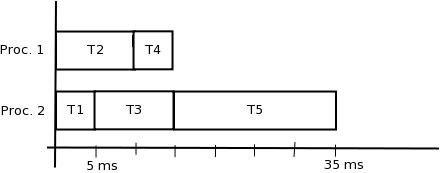
\includegraphics{taskSchedule.png}
  \caption{Task schedule}
  \label{fig:schedule}
\end{figure}
 This can also be confirmed as the minimal execution time since worst
 case propagation time is 35 ms. 

\subsection{Extract execution times for the GSM codec}

\begin{table}[h]
  \centering
  \begin{tabular}{r c c}
    \hline
    Task & First run (cycles) & Second run (cycles) \\
    \hline
    Init & 6002  & X \\
    GetInputAudio & 4576  & 4726 \\
    Preprocess & 14480  & 14258  \\
    LPC\_Analysis & 51759  & 50138 \\
    ShortTermAnalysisFilter & 92101 & 92035 \\
    LongTermPredictor2 &64820&67037\\
                       &66932&68269\\
                       &66262&67599\\
                       &66085&67093\\
    RPE\_Encoding2 &11552&11374\\
                   &10705&10632\\
                   &10667&10623\\
                   &10675&10666\\
    Add2 &1431&1445\\
         &1319&1319\\
         &1319&1319\\
         &1319&1319\\
    Encode & 3364 & 2818 \\
    Output & 3634 & 3522 \\
  \end{tabular}
  \caption{Execution times for GSM Encoder}
\end{table}


\begin{table}[h]
  \centering
  \begin{tabular}{r c c}
    \hline
    Task & First run & Second run \\
    \hline
    Init & 6086 & X \\
    GetInputAudio &1151 & 1129\\
    Decode & 2722& 2540\\
    RPE\_Decoding2 &2793&2232\\
                   &3099&3078\\
                   &3015&3015\\
                   &2979&2979\\
    LongTermSynthesis2 &4790&4608\\
                       &4608&4608\\
                       &4608&4608\\
                       &4580&4580\\
    ShortTermAnalysisFilter & 109882 & 108185\\
    PostProcessing & 7470& 7106\\
    Output & 16631& 16575\\
  \end{tabular}
  \caption{Execution times for GSM Decoder}
\end{table}


\end{document}
